\chapter{版式}

本文使用的长度单位:
1英寸 = 25.4mm = 72.27pt = 72bp。
注意 \TeX 定义的pt\nolinebreak
\footnote{pt是point的缩写,中文叫“磅”。} 和PostScript(亦即Adobe系列软件)的pt的长度不一样,
本书以 \TeX 的pt为准,PostScript的基本长度单位写为bp(big point)。

\section{纸张大小} %%%%%%%%%%%%%%%%%%%%%%%%%%%%%%

书籍的纸张大小通常异于常用的打印纸大小(A4或B5),
因此用 \LaTeX 排版书籍的第一步是设置好纸张大小。
一般常见的IT图书的开本(成品书尺寸,可以用尺子量出来)是 185mm $\times$ 230mm,
即“国际18开”;另外一种常见开本是185mm $\times$ 260mm,即“16开”。
本文以“国际18开”为例。
我们通常可以用 \fn{geometry} 宏包来设置纸张和版心尺寸,
例子见 \ref{sec:textbody} 节。

\section{版心大小} %%%%%%%%%%%%%%%%%%%%%%%%%%%%%%
\label{sec:textbody}

“版心”即正文区,不包含页眉和页脚
\footnote{这是本文的定义,也有将版心定义为包含页眉和页脚的。}。
版心的大小可以这样计算:
通常正文字号是10pt
\footnote{比五号(10.5pt)字略小,比小五号字(9pt)大。},
一行按39个汉字计算,
%\footnote{。一般不宜超过40个。}
那么行宽是 390pt。
行宽是正文字号的整数倍,这样中文间距不会无故拉宽。
行宽不宜过大,否则阅读的时候容易读串行;
也不宜过小,否则一行排不下80列代码。一般而言,
36 \textasciitilde\ 42字比较适宜,本文定为39字,数数上一行:-)。
\mybooktitle 一行是37个汉字,
因为这本书厚达600页,如果版心太宽容易影响阅读订口的文字。

对于10pt的正文字体,\LaTeX 默认的行距
\footnote{行距指的是英文基线(baseline)之间的距离,即中文汉字底部之间的距离,
不是两行之间的空白。} 是12pt,这对于英文是合适的
\footnote{因为英文文本多是小写字母,字高远小于10pt。},
但是对于中文则显得太密了。因此 \CTeX 宏包将 \fn{\bs baselinestretch} 定义为 1.3,
这样行距是\linebreak 1.3$\times$12pt = 15.6pt,阅读起来就比较顺眼了。
如果一页排34行字,那么版心的高度大约是 \nolinebreak
\footnote{这里说“大约”,因为第一行上方似乎不必留出多余的空白。} 34$\times$15.6pt=530.4pt,
本文取 530pt
\footnote{对于技术类图书,通常一个自然段不会太长,
一页之内几乎总是会遇到分段(整段代码、图表、章节标题)的情况,
因此版心高度不必严格是行距的整数倍。} 。

综上,对于39字 $\times$ 34行的版心,其尺寸是 390pt $\times$ 530pt,约合 137mm $\times$ 186mm。见下图示意。

%\vspace{1ex}
\centerline{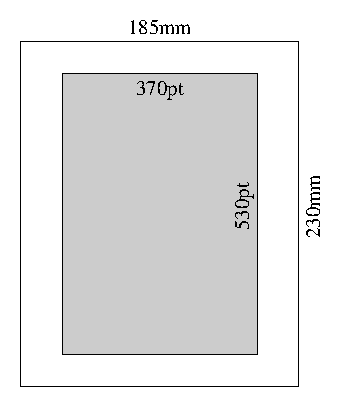
\includegraphics{paper.eps}}

知道了纸张和版心尺寸,剩下的就交给 \fn{geometry} 宏包。
例如 \myurl{examples/paper.tex}。
\begin{Codex}[label=examples/paper.tex]
\documentclass[10pt,fancyhdr,UTF8]{ctexbook}
\usepackage[centering,paperwidth=180mm,paperheight=230mm,%
            body={390pt,530pt},showframe]{geometry}
\end{Codex}

注意这里把纸张宽度设为 180mm,这是考虑到装订的位置,
这样在电脑上预览的时候左右空白更贴近实际印刷的效果。
我们也不必关心版心在纸张中的上下左右位置,居中即可,
在印刷的时候有专人负责拼版。当然在正式排版的时候要去掉 \fn{showframe} 选项。

另外,打印纸一般不会刚好和书籍开本一样大,
要想在书印出来之前感受版面效果,
可以打印在A4纸上,但需要将书页框出来,可用 \fn{crop} 宏包。
例如 \myurl{examples/paper-crop.tex}。
\begin{Code}
$ diff -u paper.tex paper-crop.tex
--- paper.tex           2012-12-29 14:03:02.000 +0800
+++ paper-crop.tex      2012-12-29 14:03:02.000 +0800
 \documentclass[10pt,fancyhdr,UTF8]{ctexbook}
 \usepackage[centering,paperwidth=180mm,paperheight=230mm,%
             body={390pt,530pt},showframe]{geometry}
+\usepackage[a4,center,frame,color=blue]{crop}
\end{Code}

\section{页眉与页脚} %%%%%%%%%%%%%%%%%%%%%%%%%%%%%%

页眉的外侧是页码,内侧是章节名称。

页脚通常可以放书名,这样即便复印其中一面也容易知道出自何处。
\subsection{各章首页}
\section{中文字体} %%%%%%%%%%%%%%%%%%%%%%%%%%%%%%

印刷用的正文字体可用方正书宋或华康简宋,
看出版社的授权情况。

屏幕阅读可用Windows的宋体或Adobe中文字体,
注意某些Adobe中文字体的标点符号位置不正确。


\section{英文字体} %%%%%%%%%%%%%%%%%%%%%%%%%%%%%%
The \LaTeX\ Font Catalogue. 
\myurl{http://www.tug.dk/FontCatalogue/}

\subsection{罗马字体}
不要使用 {\fontfamily{lmr}\selectfont Computer Modern Roman},
它笔画太细而且衬线略显夸张。
英文罗马字体一般可以选 {\fontspec{Times New Roman} Times Roman} 
\footnote{实际的字体名是 \fn{Nimbus Roman No9 L} 或 \fn{TeX Gyre Termes} 或 \fn{Times New Roman} 等。}
或 {\fontspec{URW Palladio L} Palatino}
\footnote{实际的字体名是 \fn{URW Palladio L} 或 \fn{TeX Gyre Pagella} 等。}。
例如
\begindot
\item {\fontspec{TeX Gyre Termes} C++ is a general-purpose programming language. [Times Roman]}
\item {\fontspec{TeX Gyre Pagella} C++ is a general-purpose programming language. [Palatino]}
\myenddot

\subsection{无衬线字体}

一般用于章节标题和编程语言关键字,例如“\kw{this} 指针”、
“\kw{mutable} 成员变量”。由于它出现的机会小,用什么字体其实无所谓,
默认的 \kw{Computer Modern Sans Serif} 就行。
也可以换为 {\fontspec{Nimbus Sans L} Helvetica} 
\footnote{实际的字体名是 \fn{Nimbus Sans L} 或 \fn{TeX Gyre Heros} 或 \fn{Arial} 等。}。

\subsection{等宽字体}
一般用于代码,包括变量名、类名等等。
不要使用 {\fontspec{Courier New} Courier New},它太细而且太宽。
可以用\LaTeX 默认的 {\fontspec{Latin Modern Mono} Computer Modern Typewriter}
\footnote{实际字体名是 \fn{Latin Modern Mono}。} 
或 {\fontspec{Inconsolata} Inconsolata}。后者要窄一些,但是双引号略弯。例如
\begindot
\item[] {\small \fontspec{Latin Modern Mono} printf("Hello \%s\bs n", name);} [cmtt]
\item[] {\small \fontspec[Mapping=tex-text-tt]{Inconsolata} printf("Hello \%s\bs n", name);} [Inconsolata]
\myenddot

注意如果要使用 Inconsolata 字体来排版代码,需要防止 \LaTeX 替换其中的字符,
例如 {\fontspec[Mapping=tex-text-tt]{Inconsolata} operator<<()} 变成 {\fontspec{Inconsolata} operator<<()} 等。
可以通过 \fn{fontspec} 宏包的 \fn{Mapping} 选项来做到这一点,
并搭配合适的 TECkit 映射文件
\footnote{见本文源码目录中的 \fn{tex-text-tt.map},需要用 \fn{teckit_compile} 工具编译为 \fn{{}.tec} 文件。}。


如果要排版大量Java代码,可以考虑用窄的无衬线等宽字体,如XXX。

\subsection{特殊字体}
URL可以用窄字体,以节省空间。
例如 {\fontspec{Latin Modern Mono Light Cond} Latin Modern Mono Light Cond} 或者 \myurl{PT Sans Narrow}。
特殊术语可以用稍微夸张一点的字体凸显,例如“{\fontspec{URW Gothic L} Extract Method} 重构手法”和
“{\fontspec{URW Gothic L} Observer} 模式”。

\section{整段代码}
\fn{fancyvrb} 宏包。

用 Computer Modern Typewriter 字体,版心宽度390pt时,一行可排80列。
\begin{Code}
12345678901234567890123456789012345678901234567890123456789012345678901234567890
         1         2         3         4         5         6         7         8
\end{Code}

\begin{Code}
12345678901234567890123456789012345678901234567890123456789012345678901234567890
         1         2         3         4         5         6         7         8
\end{Code}